\documentclass[table]{beamer}
\usepackage[utf8]{inputenc}
\usepackage[brazilian]{babel}
\usepackage{amsmath}
\usepackage{graphicx}
\usepackage{hyperref}
\usepackage{ragged2e}   
\usepackage{epstopdf}
\usepackage{multirow}
\usepackage{minted}
\usepackage{booktabs}

\setbeamertemplate{sidebar right}{}
\setbeamertemplate{footline}{%
\hfill\usebeamertemplate***{navigation symbols}
\hspace{1cm}\insertframenumber{}/\inserttotalframenumber}

\addtobeamertemplate{block begin}{}{\justifying}  %new code

\setbeamertemplate{footline}
{
  \leavevmode%
  \hbox{%
  \begin{beamercolorbox}[wd=.333333\paperwidth,ht=2.25ex,dp=1ex,center]{author in head/foot}%
    \usebeamerfont{author in head/foot}\insertsection
  \end{beamercolorbox}%
  \begin{beamercolorbox}[wd=.333333\paperwidth,ht=2.25ex,dp=1ex,center]{title in head/foot}%
    \usebeamerfont{title in head/foot}\insertsubsection
  \end{beamercolorbox}%
  \begin{beamercolorbox}[wd=.333333\paperwidth,ht=2.25ex,dp=1ex,right]{date in head/foot}%
    \usebeamerfont{date in head/foot}\insertshortdate{}\hspace*{2em}
    \insertframenumber{} / \inserttotalframenumber\hspace*{2ex} 
  \end{beamercolorbox}}%
  \vskip0pt%
}

\begin{document}

\begin{frame}
   \frametitle{Compiladores}
   \large
   \begin{center}
   Gramáticas Livres de Contexto e Análise Sintática
   \end{center}
   \scriptsize
   \begin{center}
      João Marcelo Uchôa de Alencar \\
      joao.marcelo@ufc.br \\
      UFC-Quixadá
   \end{center}
\end{frame}

\begin{frame}
   \tableofcontents
\end{frame}

\begin{frame}
   \frametitle{Análise Sintática}
   \begin{block}{O que é?}
      \begin{itemize}
         \item Estrutura do programa;
	 \item usa convenções e operações similares à ER;
	 \item porém admite \textbf{recursividade};
	 \item árvore sintática;
	 \item técnicas \textbf{ascendentes} e \textbf{descendentes}.
      \end{itemize}
   \end{block}
   \centering
   
\includegraphics[scale=0.7]{figuras/estudargramatica.jpeg}
\end{frame}

\section{O Processo de Análise Sintática}
\begin{frame}
   \frametitle{O Processo de Análise Sintática}
   \begin{center}
      $\text{analisador sintático}(\text{sequência de marcas}) = \text{árvore sintática}$
   \end{center}
   \begin{itemize}
      \item Em geral, o analisador sintático ativa \textit{getToken} para capturar a próxima marca sob demanda;
      \item $\text{syntaxTree} = \text{parse}()$;
      \begin{itemize}
         \item A árvore é uma estrutura dinâmica;
	 \item existem vários tipos de nós, de acordo com as regras da gramática;
	 \item registro de tamanho variável, com atributos para as próximas fases.
      \end{itemize}
      \item \textbf{recuperação de erros}: todo o código precisa ser analisado para exibir a maior quantidade de erros encontrados.
   \end{itemize}
\end{frame}

\section{Gramáticas Livres de Contexto}
\begin{frame}[fragile]
   \frametitle{Gramáticas Livres de Contexto}
   \begin{block}{Gramática}
   \textit{exp} $\to$ \textit{exp op exp} $|$ (\textit{exp}) $|$ \textbf{\textit{número}} \\
   \textit{op} $\to$ $+|-|*$ \\
   \end{block}
   \begin{block}{Expressão Regular}
   $\text{\textbf{número}} = \text{\textbf{dígito} } \text{\textbf{dígito}}^{*}$ \\
   $\text{\textbf{dígito}} = 0|1|2|3|4|5|6|7|8|9$
   \end{block}
\end{frame}

\begin{frame}
   \frametitle{Comparação com a Notação de Expressão Regular}
   \begin{itemize}
      \item ER: escolha, concatenação, repetição;
      \item gramáticas: não há a repetição da mesma forma;
      \item ER: sinal de $=$ para atribuir nome a uma expressão;
      \item gramáticas: sinal de $\to$ para definir uma regra;
      \item as ER aparecem nas regras das gramáticas.   
   \end{itemize}
\end{frame}

\begin{frame}
   \frametitle{Especificação de Regras de Gramáticas}
   \begin{itemize}
      \item Alfabeto de símbolos das gramáticas: \textbf{marcas} que representam cadeias;
      \item a cadeia \textit{if}, em uma regra, representa a marca \textbf{IF};
      \item estrutura de uma \textbf{regra}:
      \begin{itemize}
         \item nome de uma estrutura;
	 \item meta-símbolo $\to$;
	 \item símbolos do alfabeto, nome de estrutura ou o meta-símbolo $|$.
      \end{itemize}
      \item cada autor tem sua preferência nos símbolos utilizados ($=$, $:=$, $::=$, $<>$, etc) 
      \item parênteses podem ser usados para definir precedência, apesar de poderem ser substituídos por regras adicionais.
   \end{itemize}
\end{frame}

\begin{frame}
   \frametitle{Derivações e a Linguagem de uma Gramática}
   \begin{block}{Cadeias de Marcas Legais}
   As regras de gramática livres de contexto determinam o conjunto de cadeias de símbolos representando marcas consideradas sintaticamente legais dentro das estruturas de linguanges.
   \begin{itemize}
      \item $(34 - 3) * 42$ corresponde à (\textit{número} $-$ \textit{número}) $*$ \textit{número};
      \item já $(34 - 3 * 42$ não é legal, apesar das marcas serem válidas. 
   \end{itemize}
   \end{block}
   \begin{block}{Derivação}
   Sequência de substituições de nomes de estruturas por escolhas à direita das regras gramaticais. A cada passo na derivação, uma única substituição é efetuada com base em uma escolha de regra gramatical.
   \end{block}
\end{frame}

\begin{frame}
   \frametitle{Exemplo de Derivação}
   \footnotesize
   \begin{columns}
   \begin{column}{0.6\textwidth}
      \begin{enumerate}
         \item $\text{\textit{exp}} \Rightarrow \textit{exp op exp}$
	 \item \hspace{0.55cm} $\Rightarrow \text{exp op } \textbf{número}$
	 \item \hspace{0.55cm} $\Rightarrow \text{exp } * \textbf{ número}$
	 \item \hspace{0.55cm} $\Rightarrow \text{(exp) } * \textbf{ número}$
	 \item \hspace{0.55cm} $\Rightarrow \text{(exp op exp) } * \textbf{ número}$
	 \item \hspace{0.55cm} $\Rightarrow \text{(exp op \textbf{número}) } * \textbf{ número}$
	 \item \hspace{0.55cm} $\Rightarrow \text{(exp - \textbf{número}) } * \textbf{ número}$
	 \item \hspace{0.55cm} $\Rightarrow \text{(\textbf{número} - \textbf{número}) } * \textbf{ número}$
      \end{enumerate}
   \end{column}
   \begin{column}{0.4\textwidth}
      \begin{itemize}
          \item[] $[exp \to \text{\textit{exp op exp}}]$
          \item[] $[exp \to \text{\textbf{número}}]$
          \item[] $[op  \to *]$ 
          \item[] $[exp \to \text{\textit{(exp)}}]$ 
          \item[] $[exp \to \text{\textit{exp op exp}}]$ 
          \item[] $[exp \to \text{\textbf{número}}]$
          \item[] $[op  \to -]$ 
          \item[] $[exp \to \text{\textbf{número}}]$ 
      \end{itemize}
   \end{column}
   \end{columns}
\end{frame}

\begin{frame}
   \frametitle{Linguagem Definida pela Gramática}
   \begin{itemize}
      \item O conjunto de cadeias de símbolos para marcas obtidos por derivações para \textit{exp} é a \textbf{linguagem definida pela gramática};
      \item $L(G) = \{s|exp \overset{*}{\Rightarrow} s\}$
      \item cada nome de estrutura (\textit{exp, op}) define sua própria linguagem;
      \item a gramática de uma linguagem adota uma estrutura base, em geral chamada \textit{programa}, (\textbf{símbolo inicial});
      \item \textbf{símbolos não terminais}: estruturas;
      \item \textbf{símbolos terminais}: marcas.
   \end{itemize}
\end{frame}

\begin{frame}
   \frametitle{Exemplos}
   \begin{enumerate}
      \item $E \to (E)|a$, gera a linguagem $L(G) = \{{(}^{n} a {)}^{n} | n >= 0\}$;
      \item $E \to (E)$, gera a linguagem $L(G)=\{\}$;
      \item $E \to E + a | a$;
      \item \textit{declaração} $\to$ \textit{if-decl} $|$ \textbf{outra} \\
      \textit{if-decl} $\to$ \textbf{if (} \textit{exp} \textbf{)} \textit{declaração} \\
      \hspace{1.3cm} $|$ \textbf{if (} \textit{exp} \textbf{)} \textit{declaração} \textbf{else} \textit{declaração} \\
      \textit{exp} $\to$ \textbf{0} $|$ \textbf{1}
   \end{enumerate}
\end{frame}

\begin{frame}
   \frametitle{Mais Exemplos}
   \begin{enumerate}
      \item \textbf{Derivação à esquerda}: $A \to Aa|a$;
      \item \textbf{derivação à direita}: $A \to aA|a$;
      \item $A \to (A)A|\varepsilon$:
      \item \textit{declaração} $\to$ \textit{if-decl} $|$ \textbf{outra} \\
      \textit{if-decl} $\to$ \textbf{if (} \textit{exp} \textbf{)} \textit{declaração} \textit{else-parte} \\ 
      \textit{else-parte} $\to$ \textbf{else} \textit{declaração} $| \varepsilon$ \\
      \textit{exp} $\to$ \textbf{0} $|$ \textbf{1}
      \item \textit{decl-sequência} $\to$ \textit{decl} \textbf{;} \textit{decl-sequência} $|$ \textit{decl} \\
      \textit{decl} $\to$ \textbf{s}
      \item \textit{decl-sequência} $\to$ \textit{decl} \textbf{;} \textit{decl-sequência} $|\varepsilon$ \\
      \textit{decl} $\to$ \textbf{s}
   \end{enumerate}
\end{frame}

\section{Árvores}
\begin{frame}
   \frametitle{Árvores de Análise Sintática e Árvores Sintáticas Abstratas}
   Mesma cadeia final, diferentes derivações.
   \footnotesize
   \begin{columns}
   \begin{column}{0.6\textwidth}
      \begin{enumerate}
         \item $\text{\textit{exp}} \Rightarrow \textit{exp op exp}$
	 \item \hspace{0.55cm} $\Rightarrow \text{(exp) op } \textit{exp}$
	 \item \hspace{0.55cm} $\Rightarrow \text{(exp op exp)} \text{ op expr}$
	 \item \hspace{0.55cm} $\Rightarrow (\textbf{número} \text{ op exp})\text{ op exp}$
	 \item \hspace{0.55cm} $\Rightarrow (\textbf{número} - \text{exp})\text{ op exp}$
	 \item \hspace{0.55cm} $\Rightarrow (\textbf{número} - \textbf{número})\text{ op exp}$
	 \item \hspace{0.55cm} $\Rightarrow (\textbf{número} - \textbf{número}) * \text{exp}$
	 \item \hspace{0.55cm} $\Rightarrow (\textbf{número} - \textbf{número}) * \textbf{número}$
      \end{enumerate}
   \end{column}
   \begin{column}{0.4\textwidth}
      \begin{itemize}
          \item[] $[exp \to \text{\textit{exp op exp}}]$
          \item[] $[exp \to \text{\text{(exp)}}]$
          \item[] $[exp \to \text{exp op exp}]$ 
          \item[] $[exp \to \text{\textbf{número}}]$
          \item[] $[op  \to -]$ 
          \item[] $[exp \to \text{\textbf{número}}]$ 
          \item[] $[op  \to *]$ 
          \item[] $[exp \to \text{\textbf{número}}]$ 
      \end{itemize}
   \end{column}
   \end{columns}
   \normalsize
   \vspace{1.0cm}
   Precisamos de uma representação que abstraia as características essenciais de uma derivação e fatore as diferenças superficiais de ordem.
\end{frame}

\begin{frame}
   \frametitle{Árvores}
   \begin{block}{Árvore de Análise Sintática}
   Corresponde a uma derivação, com seus nós interiores rotulados por não-terminais, nós folhas rotulados por terminais e filhos de cada nó interno representando a substituição do não-terminal associado em um passo de derivação.
   \end{block}
   \hspace{1.0cm}
   \begin{columns}
   \begin{column}{0.5\textwidth}
   \begin{itemize} 
      \item[] $\textit{exp} \Rightarrow \textit{exp op exp}$
      \item[] \hspace{0.5cm} $\Rightarrow \textit{\textbf{número} op exp}$
      \item[] \hspace{0.5cm} $\Rightarrow \textit{\textbf{número} + exp}$
      \item[] \hspace{0.5cm} $\Rightarrow \textit{\textbf{número} + \textbf{número}}$
   \end{itemize}
   \end{column}
   \begin{column}{0.5\textwidth}
   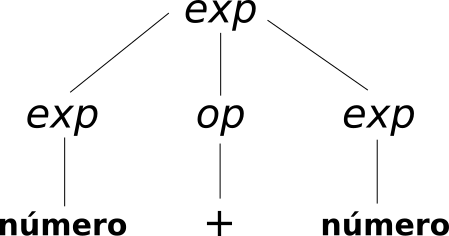
\includegraphics[width=\linewidth,height=\textheight,keepaspectratio]{figuras/primeira_arvore.png}
   \end{column}
   \end{columns}
\end{frame}

\begin{frame}
   \frametitle{Percurso em Árvores}
   Pré-ordem:
   \begin{columns}
   \begin{column}{0.5\textwidth}
   \begin{enumerate} 
      \item $\textit{exp} \Rightarrow \textit{exp op exp}$
      \item \hspace{0.5cm} $\Rightarrow \textit{\textbf{número} op exp}$
      \item \hspace{0.5cm} $\Rightarrow \textit{\textbf{número} + exp}$
      \item \hspace{0.5cm} $\Rightarrow \textit{\textbf{número} + \textbf{número}}$
   \end{enumerate}
   \end{column}
   \begin{column}{0.5\textwidth}
   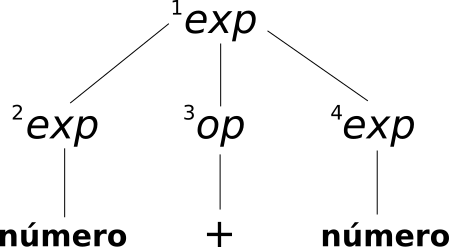
\includegraphics[width=\linewidth,height=\textheight,keepaspectratio]{figuras/segunda_arvore.png}
   \end{column}
   \end{columns}
   \vspace{1.0cm}
   Pós-ordem invertida:
   \begin{columns}
   \begin{column}{0.5\textwidth}
   \begin{enumerate} 
      \item $\textit{exp} \Rightarrow \textit{exp op exp}$
      \item \hspace{0.5cm} $\Rightarrow \textit{exp op \textbf{número}}$
      \item \hspace{0.5cm} $\Rightarrow \textit{exp + \textbf{número}}$
      \item \hspace{0.5cm} $\Rightarrow \textit{\textbf{número} + \textbf{número}}$
   \end{enumerate}
   \end{column}
   \begin{column}{0.5\textwidth}
   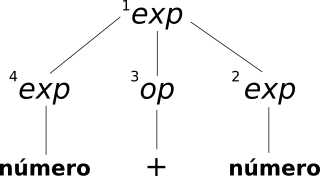
\includegraphics[width=\linewidth,height=\textheight,keepaspectratio]{figuras/terceira_arvore.png}
   \end{column}
   \end{columns}
\end{frame}

\begin{frame}
   \frametitle{Derivações e Árvores}
   \begin{block}{Correspondência}
   Uma árvore de análise sintática corresponde, em geral, a muitas derivações, as quais representam a mesma estrutura básica para as cadeias de terminais analisadas.
      \begin{itemize}
         \item \textbf{Derivação à esquerda}: não terminal mais à esquerda é substituído a cada passo da derivação; 
         \item \textbf{derivação à direita}: não terminal mais à direita é substituído a cada passo da derivação
      \end{itemize}
   \end{block}
\end{frame}

\begin{frame}
   \frametitle{Árvores  (34 - 3)*42}
   \centering
   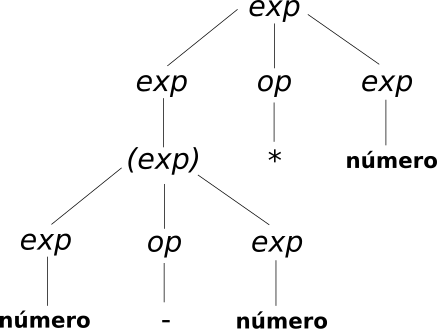
\includegraphics[scale=0.5]{figuras/quarta_arvore.png}
\end{frame}

\begin{frame}
   \frametitle{Árvores Sintáticas Abstratas}
   As árvores de análise sintática podem ser resumidas em árvores sintáticas (abstratas). Para a expressão 3 + 4: \\
   \vspace{1.0cm}
   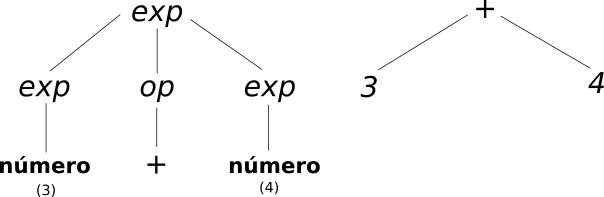
\includegraphics[width=\linewidth,height=\textheight,keepaspectratio]{figuras/arvore_abstrata.png}
\end{frame}

\begin{frame}
   \frametitle{Árvores Sintáticas Abstratas}
   \begin{block}{Construção}
   Um analisaddor sintático efetua todos os passos na árvore de análise sintática, mas, em geral, constrói apenas uma árvore sintática abstrata. 
   \end{block}
   \begin{center}
      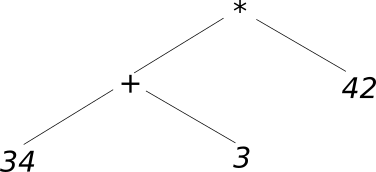
\includegraphics[scale=0.5]{figuras/segunda_arvore_abstrata.png}
   \end{center}
   \begin{block}{Sintaxe Abstrata}
   $OpExp(Mult, OpExp(Subtr, ConstExp(34), ConstExp(3)), ConstExp(42))$
   \end{block}
\end{frame}

\begin{frame}[fragile]
   \frametitle{Representação em Código}
   \begin{minted}{c}
typedef enum {Plus, Minus, Times} OpKind;
typedef enum {OpK, ConstK} ExpKind;
typedef struct streenode {
   ExpKind kind;
   OpKind op;
   struct streenode *lchild, *rchild;
   int val;
} STreeNode;
typedef STreeNode *SyntaxTree;
   \end{minted}
\end{frame}

\begin{frame}
   \frametitle{Exemplos}
   \begin{columns}
   \begin{column}{0.5\textwidth}
      \textit{declaração} $\to$ \textit{if-decl} $|$ \textbf{outra} \\
      \textit{if-decl} $\to$ \textbf{if (} \textit{exp} \textbf{)} \textit{declaração} \\
      \hspace{1.3cm} $|$ \textbf{if (} \textit{exp} \textbf{)} \textit{declaração} \textbf{else} \textit{declaração} \\
      \textit{exp} $\to$ \textbf{0} $|$ \textbf{1}
   \end{column}
   \begin{column}{0.5\textwidth}
      \textit{declaração} $\to$ \textit{if-decl} $|$ \textbf{outra} \\
      \textit{if-decl} $\to$ \textbf{if (} \textit{exp} \textbf{)} \textit{declaração} \textit{else-parte} \\ 
      \textit{else-parte} $\to$ \textbf{else} \textit{declaração} $| \varepsilon$ \\
      \textit{exp} $\to$ \textbf{0} $|$ \textbf{1}
   \end{column}
   \end{columns}
   \begin{center}
   \textbf{if (0) outra else outra}
   \end{center}
   Qual a árvore de análise sintática? Qual seria uma possível árvore sintática abstrata?
\end{frame}

\begin{frame}[fragile]
   \frametitle{Representação em Código}
   \begin{minted}{c}
typedef enum {ExpK, StmtK} NodeKind;
typedef enum {Zero, One} ExpKind;
typedef enum {IfK, OtherK} StmtKind;
typedef struct streenode {
   NodeKind kind;
   ExpKind ekind;
   StmtKind skind;
   struct streenode *test, *thenpart, *elsepart;
} STreeNode;
typedef STreeNode *SyntaxTree;
   \end{minted}
\end{frame}

\begin{frame}
   \frametitle{Mais Exemplos}
   \begin{enumerate}
      \item[] \textit{decl-sequência} $\to$ \textit{decl} \textbf{;} \textit{decl-sequência} $|$ \textit{decl} \\
      \textit{decl} $\to$ \textbf{s}
      \item[] Árvores para s;s;s ?
   \end{enumerate}
\end{frame}

\section{Ambigüidade}
\begin{frame}
   \frametitle{Ambigüidade}
   \begin{block}{Gramática}
   \textit{exp} $\to$ \textit{exp op exp} $|$ (\textit{exp}) $|$ \textbf{\textit{número}} \\
   \textit{op} $\to$ $+|-|*$ \\
   \begin{itemize}
      \item $34 - 3 * 42$
      \item Quais as derivações à esquerda e à direita?
      \item Quais as respectivas árvores?
   \end{itemize}
   \end{block}
\end{frame}

\begin{frame}
   \frametitle{Ambigüidade}
   \begin{itemize}
      \item Uma gramática que gera uma cadeia com duas árvores de análise sintática distintas é denominada \textbf{gramática ambígua};
      \item pense nela como um NFA, chega um momento na derivação que você pode fazer duas escolhas;
      \item infelizmente, diferente do caso NFA $\to$ DFA, não há transformação automática de gramática ambígua para não ambígua;
      \item soluções:
      \begin{itemize}
         \item Estabelecer uma regra externa para decidir qual caminho tomar;
	 \item alterar a gramática para eliminar a ambigüidade.
      \end{itemize}
      \item \textbf{Tradução Orientada pela Sintaxe}: escolher a árvore ou derivação que reflita melhor o significado esperado para as próximas fases da compilação.
   \end{itemize}
\end{frame}

\begin{frame}
   \frametitle{Ambigüidade}
   \begin{block}{Precedência}
   $\textit{exp} \to \textit{exp soma exp} | \textit{termo}$ \\
   $\textit{soma} \to +|-$ \\
   $\textit{termo} \to \textit{termo mult termo} | \textit{fator}$ \\
   $\textit{mult} \to *$ \\
   $\textit{fator} \to (\textit{exp}) | \textbf{número}$
   \end{block}
   \begin{block}{Associatividade}
   $\textit{exp} \to \textit{exp soma termo} | \textit{termo}$ \\
   $\textit{soma} \to +|-$ \\
   $\textit{termo} \to \textit{termo mult fator} | \textit{fator}$ \\
   $\textit{mult} \to *$ \\
   $\textit{fator} \to (\textit{exp}) | \textbf{número}$
   \end{block}
   Como ficariam as árvores para $34-3*42$ e $34-3-42$?
\end{frame}

\begin{frame}
   \frametitle{O Problema do Else Pendente}
   \textit{declaração} $\to$ \textit{if-decl} $|$ \textbf{outra} \\
   \textit{if-decl} $\to$ \textbf{if (} \textit{exp} \textbf{)} \textit{declaração} \\
   \hspace{1.3cm} $|$ \textbf{if (} \textit{exp} \textbf{)} \textit{declaração} \textbf{else} \textit{declaração} \\
   \textit{exp} $\to$ \textbf{0} $|$ \textbf{1}

   \vspace{1.0cm}
   \centering
   Qual a árvore para \textbf{if (0) if (1) outra else outra} ?
\end{frame}

\begin{frame}
   \frametitle{O Problema do Else Pendente}
   \begin{block}{Apenas casam-decl antes de um else}
   \textit{declaração} $\to$ \textit{casam-decl} $|$ \textit{sem-casam-decl} \\
   \textit{casam-decl} $\to$ \textbf{if} (\textit{exp}) \textit{casam-decl} \textbf{else} \textit{casam-decl} $|$ \textbf{outra} \\
   \textit{sem-casam-decl} $\to$ \textbf{if} (\textit{exp}) \textit{declaração} \\ 
   $|$ \textbf{if} (\textit{exp}) \textit{casam-decl} \textbf{else} \textit{sem-casam-decl} \\
   \textit{exp} $\to$ \textbf{0} $|$ \textbf{1}
   \end{block}
   \begin{itemize}
      \item Torna a gramática mais complexa;
      \item melhor determinar uma marca para finalizar o \textbf{if}.
   \end{itemize}
   \textit{if-decl} $\to$ \textbf{if} \textit{condição} \textbf{then} \textit{seq-decl} \textbf{end if} \\
   $|$ \textbf{if} \textit{condição} \textbf{then} \textit{seq-decl} \textbf{else} \textit{seq-decl} \textbf{end if}
\end{frame}

\section{EBNF}
\begin{frame}
   \frametitle{Notações Estendidas}
   \begin{block}{EBNF - Repetição e Opcionais}
      \begin{itemize}
         \item $A \to A\alpha|\beta$ vira $A \to \beta\{\alpha\}$
         \item $A \to \alpha A|\beta$ vira $A \to \{\alpha\}\beta$
	 \item $\textit{exp} \to \textit{termo } [\textit{soma exp}]$
      \end{itemize}
   \end{block}
\end{frame}

\begin{frame}
   \frametitle{Diagramas Sintáticos}
   \begin{center}
   $\textit{fator} \to (\textit{exp}) | \textbf{número}$
   \end{center}
   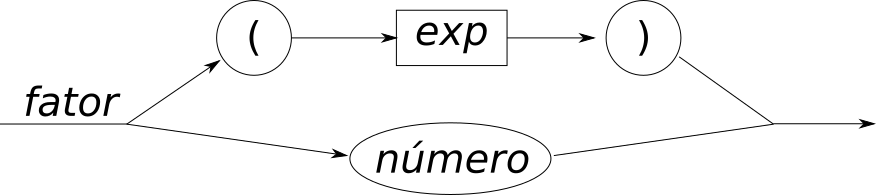
\includegraphics[width=\linewidth,height=\textheight,keepaspectratio]{figuras/diagrama_exp_numero.png}
   \begin{columns}
      \begin{column}{0.5\textwidth}
         \begin{center}
	    $A \to \{B\}$
	 \end{center}
         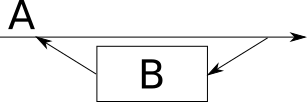
\includegraphics[width=\linewidth,height=\textheight,keepaspectratio]{figuras/diagrama_repeticao.png}
      \end{column}
      \begin{column}{0.5\textwidth}
         \begin{center}
	    $A \to [B]$
	 \end{center}
         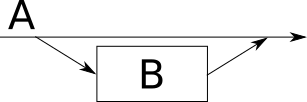
\includegraphics[width=\linewidth,height=\textheight,keepaspectratio]{figuras/diagrama_opcional.png}
      \end{column}
   \end{columns}
\end{frame}

\begin{frame}
   \frametitle{Exemplos de Diagramas Sintáticos}
   \begin{center}
   Quais são os diagramas?
   \end{center}
   \begin{columns}
      \begin{column}{0.5\textwidth}
        $\textit{declaração} \to \textit{if-decl } | \textbf{ outra}$ \\
	$\textit{if-decl} \to \textbf{if } (\textit{exp}) \textit{ declaração}$ \\
	$ | \textbf{ if } (\textit{exp}) \textit{ declaração} \textbf{ else } \textit{declaração}$  \\
	$ \textit{exp} \to \textbf{0 } | \textbf{ 1}$
      \end{column}
      \begin{column}{0.5\textwidth}
      $\textit{exp} \to \textit{termo } \{\textit{ soma termo } \}$
      $\textit{soma} \to \textbf{+ } | \textbf{ -} $
      $\textit{termo} \to \textit{fator } \{\textit{ mult fator } \}$
      $\textit{mult} \to *$
      $\textit{fator} \to (\textit{exp}) | \textbf{ número}$
      \end{column}
   \end{columns}
\end{frame}

\section{Propriedades Formais}
\begin{frame}
   \frametitle{Propriedades Formais}
   \begin{block}{Uma \textbf{gramática livre de contexto} consiste de:}
      \begin{enumerate}
         \item Um conjunto $T$ de \textbf{terminais};
	 \item um conjunto $N$ de \textbf{não-terminais} (disjunto de $T$);
	 \item um conjunto $P$ de \textbf{produções}, ou \textbf{regras gramaticais}, da forma $A \to \alpha$, em que $A$ é um elemento de $N$ e $\alpha$ é um elemento de $(T \cup N)^{*}$;
	 \item um \textbf{símbolo inicial} $S$ do conjunto $N$.
      \end{enumerate}
   \end{block}
\end{frame}

\begin{frame}
   \frametitle{Propriedades Formais}
   \begin{block}{Seja uma gramática $G=(T,N,P,S)$}
      \begin{itemize}
         \item \textbf{Passo de derivação}: $\alpha A \gamma \Rightarrow \alpha B \gamma$, em que $\alpha$ e $\gamma$ são elementos de $(T \cup N)^{*}$ e $A \to B$ pertence a $P$;
	 \item \textbf{Derivação}: $\alpha \overset{*}{\Rightarrow} \beta$ se e somente se $\alpha_{1} \Rightarrow \alpha_{2} \Rightarrow \text{...} \Rightarrow \alpha_{n-1} \Rightarrow \alpha_{n}$, com $\alpha_{1} = \alpha$ e $\alpha_{n} = \beta$;
	 \item $L(G)=\{ w \in T^{*} | \text{ existe uma derivação } S \overset{*}{\Rightarrow} w \text{ de G}  \}$
      \end{itemize}
   \end{block}
\end{frame}

\begin{frame}
   \frametitle{Propriedades Formais}
   \begin{block}{Uma árvore de análise sintática sobre $G$:}
      \begin{enumerate}
         \item Cada nó é rotulado com um terminal, um não terminal ou $\varepsilon$;
	 \item o nó raiz é rotulado coom o símbolo inicial $S$;
	 \item cada nó folha é rotulado com um terminal ou $\varepsilon$;
	 \item cada nó não folha é rotulado como um não terminal;
	 \item Se um nó com rótulo $A \in N$ tiver $n$ filhos com rótulos $X_{1}, X_{2}, ... , X_{n}$ (terminais ou não), então $A \to X_{1} X_{2} ... X_{n} \in P$ (produção).
      \end{enumerate}
   \end{block}
\end{frame}

\section{Sintaxe da TINY}
\begin{frame}
   \frametitle{Sintaxe da TINY}
   \textit{programa} $\to$ \textit{decl-sequência} \\
   \textit{decl-sequência} $\to$ \textit{decl-sequência}; \textit{declaração} $|$ \textit{declaração} \\
   \textit{declaração} $\to$ \textit{cond-decl} $|$ \textit{repet-decl} $|$ \textit{atrib-decl} $|$ \textit{leit-decl} $|$ \textit{escr-decl} \\
   \textit{cond-decl} $\to$ \textbf{if} \textit{exp} \textbf{then} \textit{decl-sequência} \textbf{end}
   $|$ \textbf{if} \text{exp} \textbf{then} \textit{decl-sequência} \textbf{else} \textit{decl-sequência} \textbf{end} \\
   \textit{repet-decl} $\to$ \textbf{repeat} \textit{decl-sequência} \textbf{until} \textit{exp} \\
   \textit{atrib-decl} $\to$ \textbf{identificador} := \textit{exp} \\
   \textit{leit-decl} $\to$ \textbf{read identificador} \\
   \textit{escr-decl} $\to$ \textbf{write} \textit{exp} \\
   \textit{exp} $\to$ \textit{exp-simples comp-op exp-simples} $|$ \textit{exp-simples} \\
   \textit{comp-op} $\to <|=$ \\
   \textit{exp-simples} $\to$ \textit{exp-simples soma termo} $|$ \textit{termo} \\
   \textit{soma} $\to +|-$ \\
   \textit{termo} $\to$ \textit{termo mult fator} $|$ \textit{fator} \\
   \textit{mult} $\to *|/$ \\
   \textit{fator} $\to$ \textit{(exp)} $|$ \textbf{número} $|$ \textbf{identificador}
\end{frame}

\begin{frame}[fragile]
   \frametitle{Estruturas da Árvore Sintática Abstrata da TINY}
   \footnotesize
   \begin{minted}{c}
typedef enum {StmtK, ExpK} NodeKind;
typedef enum {IfK, RepeatK, AssignK, ReadK, WriteK} 
             StmtKind;
typedef enum {OpK, ConstK, IdK} ExpKind;
/* ExpType é utilizado para verificação de tipos. */	     
typedef enum {Void, Integer, Boolean} ExpType;
#define MAXCHILDREN 3
typedef struct treeNode {
   struct treeNode *child[MAXCHILDREN];
   struct treeNode *sibling;
   int lineno;
   NodeKind nodekind;
   union { StmtKind stmt; ExpKind exp;} kind;
   union { TokenType op;
           int val;
	   char *name; } attr;
   ExpType type;
} TreeNode;
   \end{minted}
\end{frame}

\begin{frame}[fragile]
   \frametitle{Estruturas da Árvore Sintática Abstrata da TINY}
   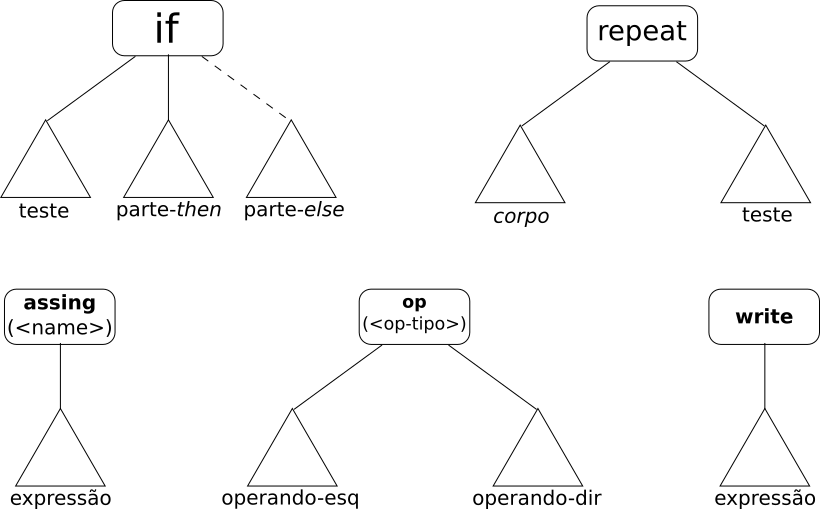
\includegraphics[width=\linewidth,height=\textheight,keepaspectratio]{figuras/diagrama_tiny.png}
\end{frame}

\begin{frame}[fragile]
   \frametitle{Programa Exemplo na Linguagem TINY}
   \begin{minted}{pascal}
{
   Programa de exemplo na 
   linguagem TINY - computa o fatorial
}
read x; {entrada de um inteiro}
if 0 < x then { não calcula se x <= 0}
   fact := 1;
   repeat
      fact := fact * x;
      x := x - 1;
   until x = 0;
   write fact {saída do fatorial de x}
end
   \end{minted}
   Qual seria a árvore sintática abstrata baseada nas estruturas?
\end{frame}

\begin{frame}
   \frametitle{Fim}
   Dúvidas?
\end{frame}

\end{document}
